\documentclass[11pt]{article}
\setlength\parindent{10pt}
\usepackage{booktabs, natbib, amsmath, amssymb, mathrsfs, tabularx, makecell}
\usepackage[margin=1in]{geometry}
\usepackage{caption}
\usepackage{subcaption}
\usepackage{authblk}
\usepackage{tikz}
\usetikzlibrary{positioning, arrows.meta, calc}
\usepackage{hyperref}
\usepackage{graphicx}
\pagestyle{plain}

\captionsetup[table]{skip=10pt}
\captionsetup[figure]{skip=10pt}

\title{Evidence Based Assessment of Research Influence:\\
A Global Spectral Ranking across Scientific Fields}

\author[1]{Domingo Docampo}
\author[2]{Lawrence Cram}

\affil[1]{Atlantic Research Center for Information and Communication Technologies \newline
University of Vigo, Vigo, Spain}
\affil[2]{Research School of Physics, Australian National University, Canberra, 2600, ACT, Australia \newline
Charles Darwin University, Brinkin, 0810, NT, Australia}

\date{\today}

\begin{document}
\maketitle

\begin{abstract}
National research evaluation frameworks are transitioning from burdensome, submission-heavy assessment exercises toward agile, data-driven systems grounded in transparent global bibliometrics. However, conventional citation metrics suffer from systemic defects: raw volume bias that rewards scale over quality, reliance on opaque journal impact factors, and vulnerability to metric gaming. Here we introduce an evidence-based framework for national research evaluation utilizing a bipartite spectral ranking model. Modeling scientific influence as a mutual reinforcement network between publishing channels (sources, $\mathcal{S}$) and research institutions ($\mathcal{I}$), we apply a one-mode Breiger projection to derive an intrinsic, size-independent prestige intensity metric ($v$), calibrated such that the global average across any discipline is exactly unity ($1.0$). We ground this global model in national policy frameworks by establishing an audited concordance (AREA5) bridging the 23 two-digit divisions of the Australian ANZSRC FOR 2020 standard and OpenAlex's machine-learned topic hierarchy, preserving computing and mathematical sciences as an independent analytical pillar and properly aligning veterinary science with agriculture. Evaluating all 42 Australian Higher Education Providers across the 2020--2024 census window reveals that research intensity flourishes across diverse university mission groups, demonstrating that specialized technological universities (e.g., Swinburne and UTS in computing and engineering) and targeted institutions (e.g., ACU in social sciences and nursing) achieve world-leading excellence comparable to the comprehensive Group of Eight. Extensive geopolitical bloc and parameter sensitivity analyses confirm that institutional prestige rankings remain remarkably robust ($\rho_s > 0.98$ under OECD+G20 restrictions). The bipartite spectral framework provides higher education authorities with an open, reproducible, and equitable instrument for evidence-based research evaluation.
\end{abstract}

% ---------------------------------------------------------------
\section{Introduction}
\label{sec:introduction}
% ---------------------------------------------------------------

National research evaluation systems face an enduring challenge: how to assess the quality, influence, and impact of scholarly output across diverse institutions equitably, transparently, and without imposing unsustainable administrative burdens. In Australia, the Excellence in Research for Australia (ERA) framework, established in 2010 by the Australian Research Council \citep{arc2019era}, relied on comprehensive institutional data submissions evaluated through a hybrid of peer review panels and citation benchmarks. Over five rounds, ERA successfully mapped the national research landscape but incurred substantial direct compliance costs for universities. Following the independent review of the ARC Act in 2023 \citep[\textit{Trusting Australia's Ability},][]{sheil2023trusting} and the Australian Universities Accord \citep{accord2024final}, the Australian Government announced the discontinuation of the decennial ERA cycle in favor of developing a modern, data-driven national research assessment system that harnesses transparent global bibliometric data.

Similar transitions are underway internationally. The UK's Research Excellence Framework (REF) is continually reassessing the balance between expert peer assessment and algorithmic indicators \citep{wilsdon2015metric}, while international university league tables continue to proliferate. However, conventional bibliometric indicators remain fraught with systemic limitations when deployed for national evaluation:

\begin{enumerate}
    \item \textbf{Size and Volume Bias}: Raw publication counts and aggregate citation totals systematically advantage large, multi-faculty institutions over smaller, specialized, or regional universities \citep{docampo2014internal, docampo2015effect, docampo2017academic}. Size-dependent measures reward scale rather than research intensity or quality per output.
    \item \textbf{Journal Impact Factor (JIF) Fallacy}: Assigning value to an individual paper based exclusively on the journal in which it appears ignores the highly skewed distribution of citations within journals and overlooks the prestige and intellectual environment of the authoring institutions \citep{seglen1997why, hicks2015leiden}.
    \item \textbf{Field Incommensurability}: Citation densities, publication velocity, and co-authorship customs differ drastically between fields---for example, between clinical medicine and the humanities. Comparing raw citation counts across fields without rigorous normalization produces severe disciplinary distortions.
    \item \textbf{Gaming and Insularity}: Unipartite citation measures can be distorted by self-citation networks, citation clubs, and regional insularity, obscuring genuine scholarly influence.
\end{enumerate}

To overcome these structural defects, this paper presents an evidence-based framework for national research evaluation built upon a \textbf{bipartite spectral ranking model} \citep{docampo2025screening}. Instead of viewing journals or institutions in isolation, our approach formalizes scientific influence as a mutual reinforcement network between publishing channels (sources, $\mathcal{S}$) and research institutions ($\mathcal{I}$). High-prestige journals are those cited by leading research institutions, and high-prestige institutions are those that publish frequently in, and are cited by, influential journals. 

By applying a one-mode Breiger projection \citep{breiger1974duality} and solving for the dominant Perron eigenvector, we derive an intrinsic, size-independent influence intensity metric, $v$, scaled such that the global average across any discipline is exactly $1.0$. An institution with $v_I = 2.0$ in a given field produces research that attracts twice the global baseline prestige per unit of published work, irrespective of whether the university publishes 100 or 10,000 papers.

Furthermore, we ground this global model directly in national policy frameworks by creating an explicit concordance between the open scholarly graph provided by OpenAlex \citep{priem2022openalex} and the Australian and New Zealand Standard Research Classification \citep[ANZSRC 2020;][]{anzsrc2020} Fields of Research (FOR). We organize this evaluation at two complementary tiers:
\begin{itemize}
    \item A macro-level \textbf{5 Broad Research Areas (AREA5)}---separating computing and mathematical sciences as an independent analytical pillar from physical sciences and engineering, and properly aligning veterinary science with agricultural and animal sciences.
    \item A meso-level \textbf{26-discipline field tier}, mapping directly to 2-digit ANZSRC FOR divisions.
\end{itemize}

Applying this model to all 42 Australian Higher Education Providers (HEPs) across the 2020--2024 census window reveals distinct institutional profiles, demonstrating that research intensity flourishes across diverse mission groups---including the Group of Eight (Go8), the Australian Technology Network (ATN), the Innovative Research Universities (IRU), and Regional Universities Network (RUN). Finally, extensive sensitivity and geopolitical bloc analyses demonstrate that the spectral ranking is remarkably robust against shifts in citation boundaries and parameter variations.

% ---------------------------------------------------------------
\section{Bipartite Spectral Ranking Methodology}
\label{sec:spectral_ranking}
% ---------------------------------------------------------------

\subsection{Bipartite Network Formulation}

Traditional bibliometrics model citation graphs as unipartite networks—either direct journal-to-journal citation matrices or direct institution-to-institution citation exchanges. However, scientific communication fundamentally operates as a bipartite interaction between two distinct types of entities:
\begin{itemize}
    \item \textbf{Publishing Channels / Sources ($\mathcal{S}$)}: Peer-reviewed journals, book series, and selective conference proceedings ($|\mathcal{S}| = N_S$).
    \item \textbf{Research Institutions ($\mathcal{I}$)}: Universities, hospitals, and public research agencies ($|\mathcal{I}| = N_U$).
\end{itemize}

Articles are authored by researchers affiliated with institutions $\mathcal{I}$ and published in sources $\mathcal{S}$. When article $A$ (published in source $s \in \mathcal{S}$ with author affiliations $i \in \mathcal{I}$) cites article $B$ (published in source $s' \in \mathcal{S}$ with author affiliations $i' \in \mathcal{I}$), this citation generates two complementary cross-entity links:
\begin{enumerate}
    \item A citation link from citing source $s$ to cited institution $i'$.
    \item A citation link from citing institution $i$ to cited source $s'$.
\end{enumerate}

\begin{figure}[htbp]
\centering
\resizebox{0.92\textwidth}{!}{%
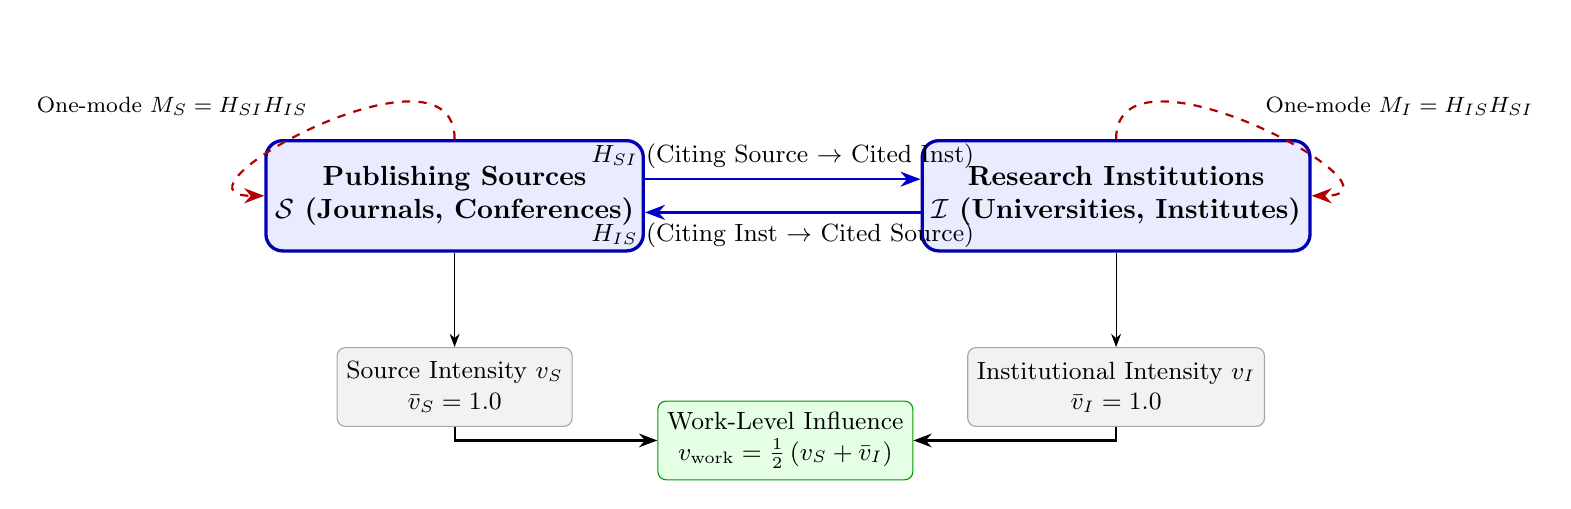
\begin{tikzpicture}[
    node distance=2.8cm and 3.5cm,
    entity/.style={rectangle, rounded corners=6pt, draw=blue!70!black, fill=blue!8, very thick, minimum width=3.2cm, minimum height=1.4cm, align=center, font=\bfseries},
    process/.style={rectangle, draw=gray!70, fill=gray!10, rounded corners=3pt, minimum width=2.6cm, minimum height=1.0cm, align=center, font=\small},
    arrow/.style={-{Stealth[scale=1.1]}, thick, draw=blue!80!black},
    darrow/.style={-{Stealth[scale=1.1]}, thick, dashed, draw=red!70!black}
]

% Entities
\node[entity] (sources) {Publishing Sources\\$\mathcal{S}$ (Journals, Conferences)};
\node[entity, right=of sources] (insts) {Research Institutions\\$\mathcal{I}$ (Universities, Institutes)};

% Cross citation transitions
\draw[arrow] ([yshift=6pt]sources.east) -- node[above, font=\small] {$H_{SI}$ (Citing Source $\to$ Cited Inst)} ([yshift=6pt]insts.west);
\draw[arrow] ([yshift=-6pt]insts.west) -- node[below, font=\small] {$H_{IS}$ (Citing Inst $\to$ Cited Source)} ([yshift=-6pt]sources.east);

% Breiger Projection loops
\draw[darrow] (sources.north) .. controls +(up:1.4cm) and +(left:1.4cm) .. node[above left, font=\footnotesize] {One-mode $M_S = H_{SI} H_{IS}$} (sources.west);
\draw[darrow] (insts.north) .. controls +(up:1.4cm) and +(right:1.4cm) .. node[above right, font=\footnotesize] {One-mode $M_I = H_{IS} H_{SI}$} (insts.east);

% Resulting metrics below
\node[process, below=1.2cm of sources] (vs) {Source Intensity $v_S$\\$\bar{v}_S = 1.0$};
\node[process, below=1.2cm of insts] (vi) {Institutional Intensity $v_I$\\$\bar{v}_I = 1.0$};

\draw[-{Stealth}] (sources.south) -- (vs);
\draw[-{Stealth}] (insts.south) -- (vi);

% Synthesis
\node[process, fill=green!10, draw=green!60!black, below=2.6cm of $(sources)!0.5!(insts)$] (vwork) {Work-Level Influence\\$v_{\text{work}} = \frac{1}{2}\left(v_S + \bar{v}_I\right)$};

\draw[-{Stealth}, thick] (vs.south) |- (vwork.west);
\draw[-{Stealth}, thick] (vi.south) |- (vwork.east);

\end{tikzpicture}%
}
\caption{Conceptual architecture of the bipartite source/institution spectral ranking model. Mutual reinforcement between publishing sources $\mathcal{S}$ and research institutions $\mathcal{I}$ yields one-mode Breiger projections ($M_S, M_I$), from which size-independent prestige intensities ($v_S, v_I$) and work-level status ($v_{\text{work}}$) are derived.}
\label{fig:bipartite_schematic}
\end{figure}

Let $C_{SI}$ be the raw $N_S \times N_U$ cross-citation matrix where element $c_{s, i'}$ records the aggregate volume of citations from source $s$ to institution $i'$. Conversely, let $C_{IS}$ be the $N_U \times N_S$ cross-citation matrix where element $c_{i, s'}$ records the volume of citations from institution $i$ to source $s'$.

\subsection{Fractional Weighting and Cross-Disciplinary Conservation}

To prevent distortion from hyper-authored papers and multi-institution consortia, fractional weighting is applied at both the institution and disciplinary levels:
\begin{enumerate}
    \item \textbf{Author-Fractional Institutional Weight ($w_{\text{inst}}$)}: For an article with $n_a$ authors, where author $k$ has $n_{i,k}$ institutional affiliations, the institutional weight assigned to institution $j$ is:
    \begin{equation}
        w_{\text{inst}}(j) = \sum_{k=1}^{n_a} \frac{\mathbb{I}(j \in \text{Affil}_k)}{n_a \cdot n_{i,k}}, \quad \sum_{j \in \mathcal{I}} w_{\text{inst}}(j) = 1
    \end{equation}
    Papers with consortium authorship exceeding 29 authors are excluded to avoid massive particle-physics or genomics consortium distortions.
    \item \textbf{Disciplinary Field Weight ($w_{\text{field}}$)}: When an article is assigned multiple topics across disciplines, the weight for field $X$ is normalized by the total topic confidence scores:
    \begin{equation}
        w_{\text{field}}(X) = \frac{\sum_{t \in X} \text{score}(t)}{\sum_{t} \text{score}(t)}, \quad \sum_{X} w_{\text{field}}(X) = 1
    \end{equation}
    An edge between citer $A$ and cited work $B$ in field $X$ receives weight $e_{AB} = \frac{1}{2}(w_{\text{field}}(A, X) + w_{\text{field}}(B, X))$, preserving total citation mass globally.
\end{enumerate}

\subsection{Row Normalization and Breiger Projection}

Raw citation matrices are row-normalized to obtain row-stochastic transition operators $H_{SI}$ and $H_{IS}$:
\begin{equation}
    H_{SI} = D_{S}^{-1} C_{SI}, \quad H_{IS} = D_{I}^{-1} C_{IS}
\end{equation}
where $D_S$ and $D_I$ are diagonal degree matrices whose entries are row sums of $C_{SI}$ and $C_{IS}$ (with zero/dangling rows handled through uniform prior redistribution).

Rather than solving a block-coupled $2 \times 2$ system directly, we utilize the classic Breiger one-mode dual projection \citep{breiger1974duality}. The round-trip operator for sources, $M_S$, and institutions, $M_I$, are defined as:
\begin{equation}
    M_S = H_{SI} H_{IS} \in \mathbb{R}^{N_S \times N_S}, \quad M_I = H_{IS} H_{SI} \in \mathbb{R}^{N_U \times N_U}
\end{equation}
$M_S$ represents a two-step citation walk: from a citing source to a cited institution, and then from that institution to the sources it cites. In network terms, this captures the mutual reinforcement principle pioneered by \citet{katz1953new}, \citet{bonacich1987power}, and \citet{kleinberg1999authoritative}, extended here to a bipartite scholarly setting related to invariant citation flows \citep{page1999pagerank, bergstrom2008eigenfactor}. $M_S$ is row-stochastic and, for connected citation graphs, primitive with spectral radius $\lambda_1 = 1.0$.

\subsection{Eigensolve and Normalized Prestige Intensity \texorpdfstring{($v$)}{(v)}}

The dominant Perron eigenvector $\pi_S$ satisfying $\pi_S = M_S^T \pi_S$ (normalized such that $\sum_{s} \pi_S(s) = 1$) yields the global prestige vector over publishing sources. The institutional prestige vector $\pi_I$ is obtained directly via:
\begin{equation}
    \pi_I = H_{SI}^T \pi_S, \quad \sum_{i} \pi_I(i) = 1
\end{equation}
The spectral gap, $1 - |\lambda_2|$, serves as a diagnostic of graph connectivity and community mixing. Across all fields in our data, $|\lambda_2| \le 0.67$, ensuring rapid geometric convergence and well-separated principal prestige dimensions.

Raw prestige $\pi$ scales with publication volume: an institution that publishes 1,000 papers naturally accumulates more total prestige than one publishing 50 papers \citep{docampo2014internal}. To obtain a \textbf{size-independent research quality intensity}, following \citet{docampo2025screening}, we divide prestige by the institution's weighted publication output ($w_I$) and scale by entity count:
\begin{equation}
    v_S(s) = \frac{\pi_S(s)}{w_S(s)} \cdot N_S, \quad v_I(i) = \frac{\pi_I(i)}{w_I(i)} \cdot N_U
\end{equation}
By construction, the weighted mean across all qualifying entities is exactly unity:
\begin{equation}
    \bar{v}_S = \frac{1}{N_S} \sum_{s \in \mathcal{S}} v_S(s) \cdot w_S(s) = 1.0, \quad \bar{v}_I = \frac{1}{N_U} \sum_{i \in \mathcal{I}} v_I(i) \cdot w_I(i) = 1.0
\end{equation}
Values of $v > 1.0$ indicate performance above the global baseline; values $v < 1.0$ denote performance below the global mean.

Finally, each published article inherits a dual status reflecting both its publication venue and its authorial institutional pedigree:
\begin{equation}
    v_{\text{work}} = \frac{1}{2}\left( v_S + \frac{1}{|\mathcal{I}_{\text{work}}|} \sum_{i \in \mathcal{I}_{\text{work}}} v_I(i) \right)
\end{equation}
This formulation provides a size-independent, field-normalized, and tamper-resistant assessment metric suitable for national evaluation.

% ---------------------------------------------------------------
\section{Data Corpus and National Disciplinary Taxonomy}
\label{sec:data}
% ---------------------------------------------------------------

\subsection{OpenAlex Snapshot and Corpus Filtering}

The empirical foundation for this study is built from a global snapshot of OpenAlex citation metadata \citep{priem2022openalex} encompassing all scholarly works published between 2000 and 2025, with our primary national research evaluation focusing on the five-year census window \textbf{2020--2024}. 

To construct an authoritative corpus, we extract a master relational table, \texttt{flat\_works}, containing approximately 261.4 million records structured at the $( \text{work} \times \text{institution} \times \text{subfield} )$ level. The following rigorous quality filters are applied:
\begin{itemize}
    \item \textbf{Scholarly Work Types}: Expanded to eight primary peer-reviewed formats: \textit{article, review, book, book-chapter, dissertation, letter, preprint, report}.
    \item \textbf{Integrity and Completeness}: Filtered to non-retracted works, excluding paratext (editorials, front matter, tables of contents), and requiring $\text{referenced\_works\_count} \ge 1$.
    \item \textbf{Consortium Threshold}: Works with $\text{authors\_count} > 29$ are excluded to eliminate mega-authored consortium publications whose author credits obscure institutional responsibility.
    \item \textbf{Title Deduplication}: Normalized title deduplication ensures preprints and subsequent formal journal publications do not double-count citation linkages.
    \item \textbf{Institution Types}: Restricted to research-performing organizational classes: \textit{education, nonprofit, government, healthcare, and other}. Clinical research institutes and university teaching hospitals are explicitly captured under the \textit{healthcare} designation.
\end{itemize}

\subsection{Retention Thresholds \texorpdfstring{($\tau$)}{(tau)}}

To ensure statistical stability and avoid spurious eigenvalues driven by singleton or transient entities, minimum activity thresholds are enforced:
\begin{itemize}
    \item $\tau_S = 10.0$ weighted works per year for publishing sources (50.0 weighted works over the 2020--2024 window).
    \item $\tau_U = 10.0$ weighted works per year for research institutions (50.0 weighted works over the 2020--2024 window).
\end{itemize}
Because thresholds are defined in weighted works per year, the qualification criterion remains invariant to the length of the census window.

\subsection{The AREA5 Concordance: Bridging OpenAlex and ANZSRC FOR 2020}

A central innovation of this framework is establishing a direct, audited mapping between OpenAlex's global topic hierarchy and the Australian and New Zealand Standard Research Classification \citep[ANZSRC 2020;][]{anzsrc2020}. 

Rather than adopting the four-domain model of OpenAlex (which submerges computer science and mathematics into the physical sciences) or relying on the proprietary five-superfield model of the CWTS Leiden Ranking \citep{waltman2012new} (which places veterinary science into human biomedical health), we establish a unified \textbf{5 Broad Research Areas (AREA5)} framework. This taxonomy is explicitly grounded in the 23 two-digit divisions of ANZSRC FOR 2020 and linked directly to OpenAlex's 26 fields, as documented in Table~\ref{tab:area5_concordance}.

\begin{table}[htbp]
\centering
\small
\caption{Concordance of the Five Broad Research Areas (AREA5) with Australian ANZSRC 2020 Divisions and OpenAlex Fields.}
\label{tab:area5_concordance}
\begin{tabularx}{\textwidth}{l >{\raggedright\arraybackslash}p{3.8cm} >{\raggedright\arraybackslash}p{2.6cm} >{\raggedright\arraybackslash}X}
\toprule
\textbf{Code} & \textbf{Broad Discipline} & \textbf{ANZSRC FOR 2020 (2-digit)} & \textbf{OpenAlex Fields} \\
\midrule
MCS & Mathematics, Computing and Information Sciences & 46, 49 & 17 CompSci, 26 Maths \\
PSE & Physical Sciences and Engineering & 33, 34, 40, 51 & 15 ChemEng, 16 Chemistry, 21 Energy, 22 Engineering, 25 Materials, 31 Physics \\
LES & Life, Agricultural and Environmental Sciences & 30, 31, 37, 41 & 11 Ag\&Bio, 13 Biochem, 19 Earth, 23 EnvSci, 24 Immunol, 34 Vet \\
BHS & Biomedical and Health Sciences & 32, 42 & 27 Medicine, 28 Neurosci, 29 Nursing, 30 Pharma, 35 Dentistry, 36 HealthProf \\
SSH & Social Sciences, Humanities, Arts and Business & 35, 36, 38, 39, 43, 44, 47, 48, 50, 52 & 12 Arts\&Hum, 14 Business, 18 Decision, 20 Economics, 32 Psychology, 33 SocSci \\
IND & Indigenous Studies & 45 & \textit{Recognized national priority, zero-populated} \\
\bottomrule
\end{tabularx}
\end{table}


Two key boundary definitions warrant emphasis:
\begin{enumerate}
    \item \textbf{Mathematics and Computing (MCS)}: Information and Computing Sciences (Division 46) and Mathematical Sciences (Division 49) form an autonomous macro-discipline. This reflects their distinct publication mechanisms (where top computer science conferences carry equal or greater prestige than journals) and prevents their intensity from being obscured within heavy industrial engineering or chemistry.
    \item \textbf{Veterinary Science (LES)}: In strict concordance with ANZSRC Division 30 (\textit{Agricultural, Veterinary and Food Sciences}), veterinary science is united with animal biology and agricultural ecology within Life and Earth Sciences (LES), rather than combined with human clinical medicine and hospital epidemiology in Biomedical and Health Sciences (BHS).
    \item \textbf{Indigenous Studies (IND)}: Division 45 is an essential national research priority. Because machine-learned global topic models do not currently distinguish a standalone Indigenous branch from the underlying academic disciplines through which it is expressed, Division 45 is carried as an explicitly recognized, zero-populated category in global data rather than silently discarded.
\end{enumerate}

\subsection{Corpus Scale and Spectral Health}

Table~\ref{tab:corpus_summary} reports the scale of the retained bipartite network and the corresponding eigensolve diagnostics across each of the five broad disciplines.

\begin{table}[htbp]
\centering
\small
\caption{Corpus Scale and Spectral Properties across the Five Broad Disciplines (2020--2024 Census Window).}
\label{tab:corpus_summary}
\begin{tabularx}{\textwidth}{l >{\raggedright\arraybackslash}X r r ccc}
\toprule
\textbf{Code} & \textbf{Broad Discipline} & \textbf{Sources ($N_S$)} & \textbf{Institutions ($N_U$)} & $\lambda_1$ & $\lambda_2$ & \textbf{Spectral Gap} \\
\midrule
MCS & Maths \& Computing & 3,896 & 4,173 & 0.9998 & 0.5588 & 0.4412 \\
PSE & Physical \& Engineering & 7,137 & 6,025 & 0.9999 & 0.6670 & 0.3330 \\
LES & Life \& Earth Sciences & 9,099 & 7,505 & 1.0000 & 0.4134 & 0.5866 \\
BHS & Biomedical \& Health & 11,989 & 10,821 & 1.0000 & 0.5824 & 0.4176 \\
SSH & Social Sci \& Humanities & 17,354 & 7,942 & 0.9999 & 0.6030 & 0.3970 \\
\bottomrule
\end{tabularx}
\end{table}


Across all five areas, the qualifying network encompasses thousands of selective sources ($N_S$ from 3,896 in MCS to 17,354 in SSH) and world research institutions ($N_U$ from 4,173 in MCS to 10,821 in BHS). In every case, the dominant eigenvalue $\lambda_1$ converges to $1.0000 \pm 0.0002$ under ARPACK Arnoldi iteration. 

Crucially, the spectral gap ($1 - \lambda_2$) ranges between $0.3330$ and $0.5866$, confirming that the bipartite cross-citation graphs are strongly primitive, free of disconnected sub-components, and characterized by rapid geometric convergence of the prestige distribution.

% ---------------------------------------------------------------
\section{Empirical Results: National Research Evaluation in Australia}
\label{sec:results}
% ---------------------------------------------------------------

\subsection{Institutional Profiles of Australian Higher Education Providers}

Applying the bipartite spectral ranking model across all 42 Australian Higher Education Providers (HEPs) provides a comprehensive, size-independent mapping of Australian university research influence. 

Figure~\ref{fig:hep_heatmap} displays the full influence heatmap of Australian universities across all 26 OpenAlex disciplines for the 2020--2024 window, while Table~\ref{tab:hep_summary} reports institutional prestige scores ($v_I$) aggregated into the five canonical AREA5 broad disciplines.

\begin{figure}[htbp]
\centering
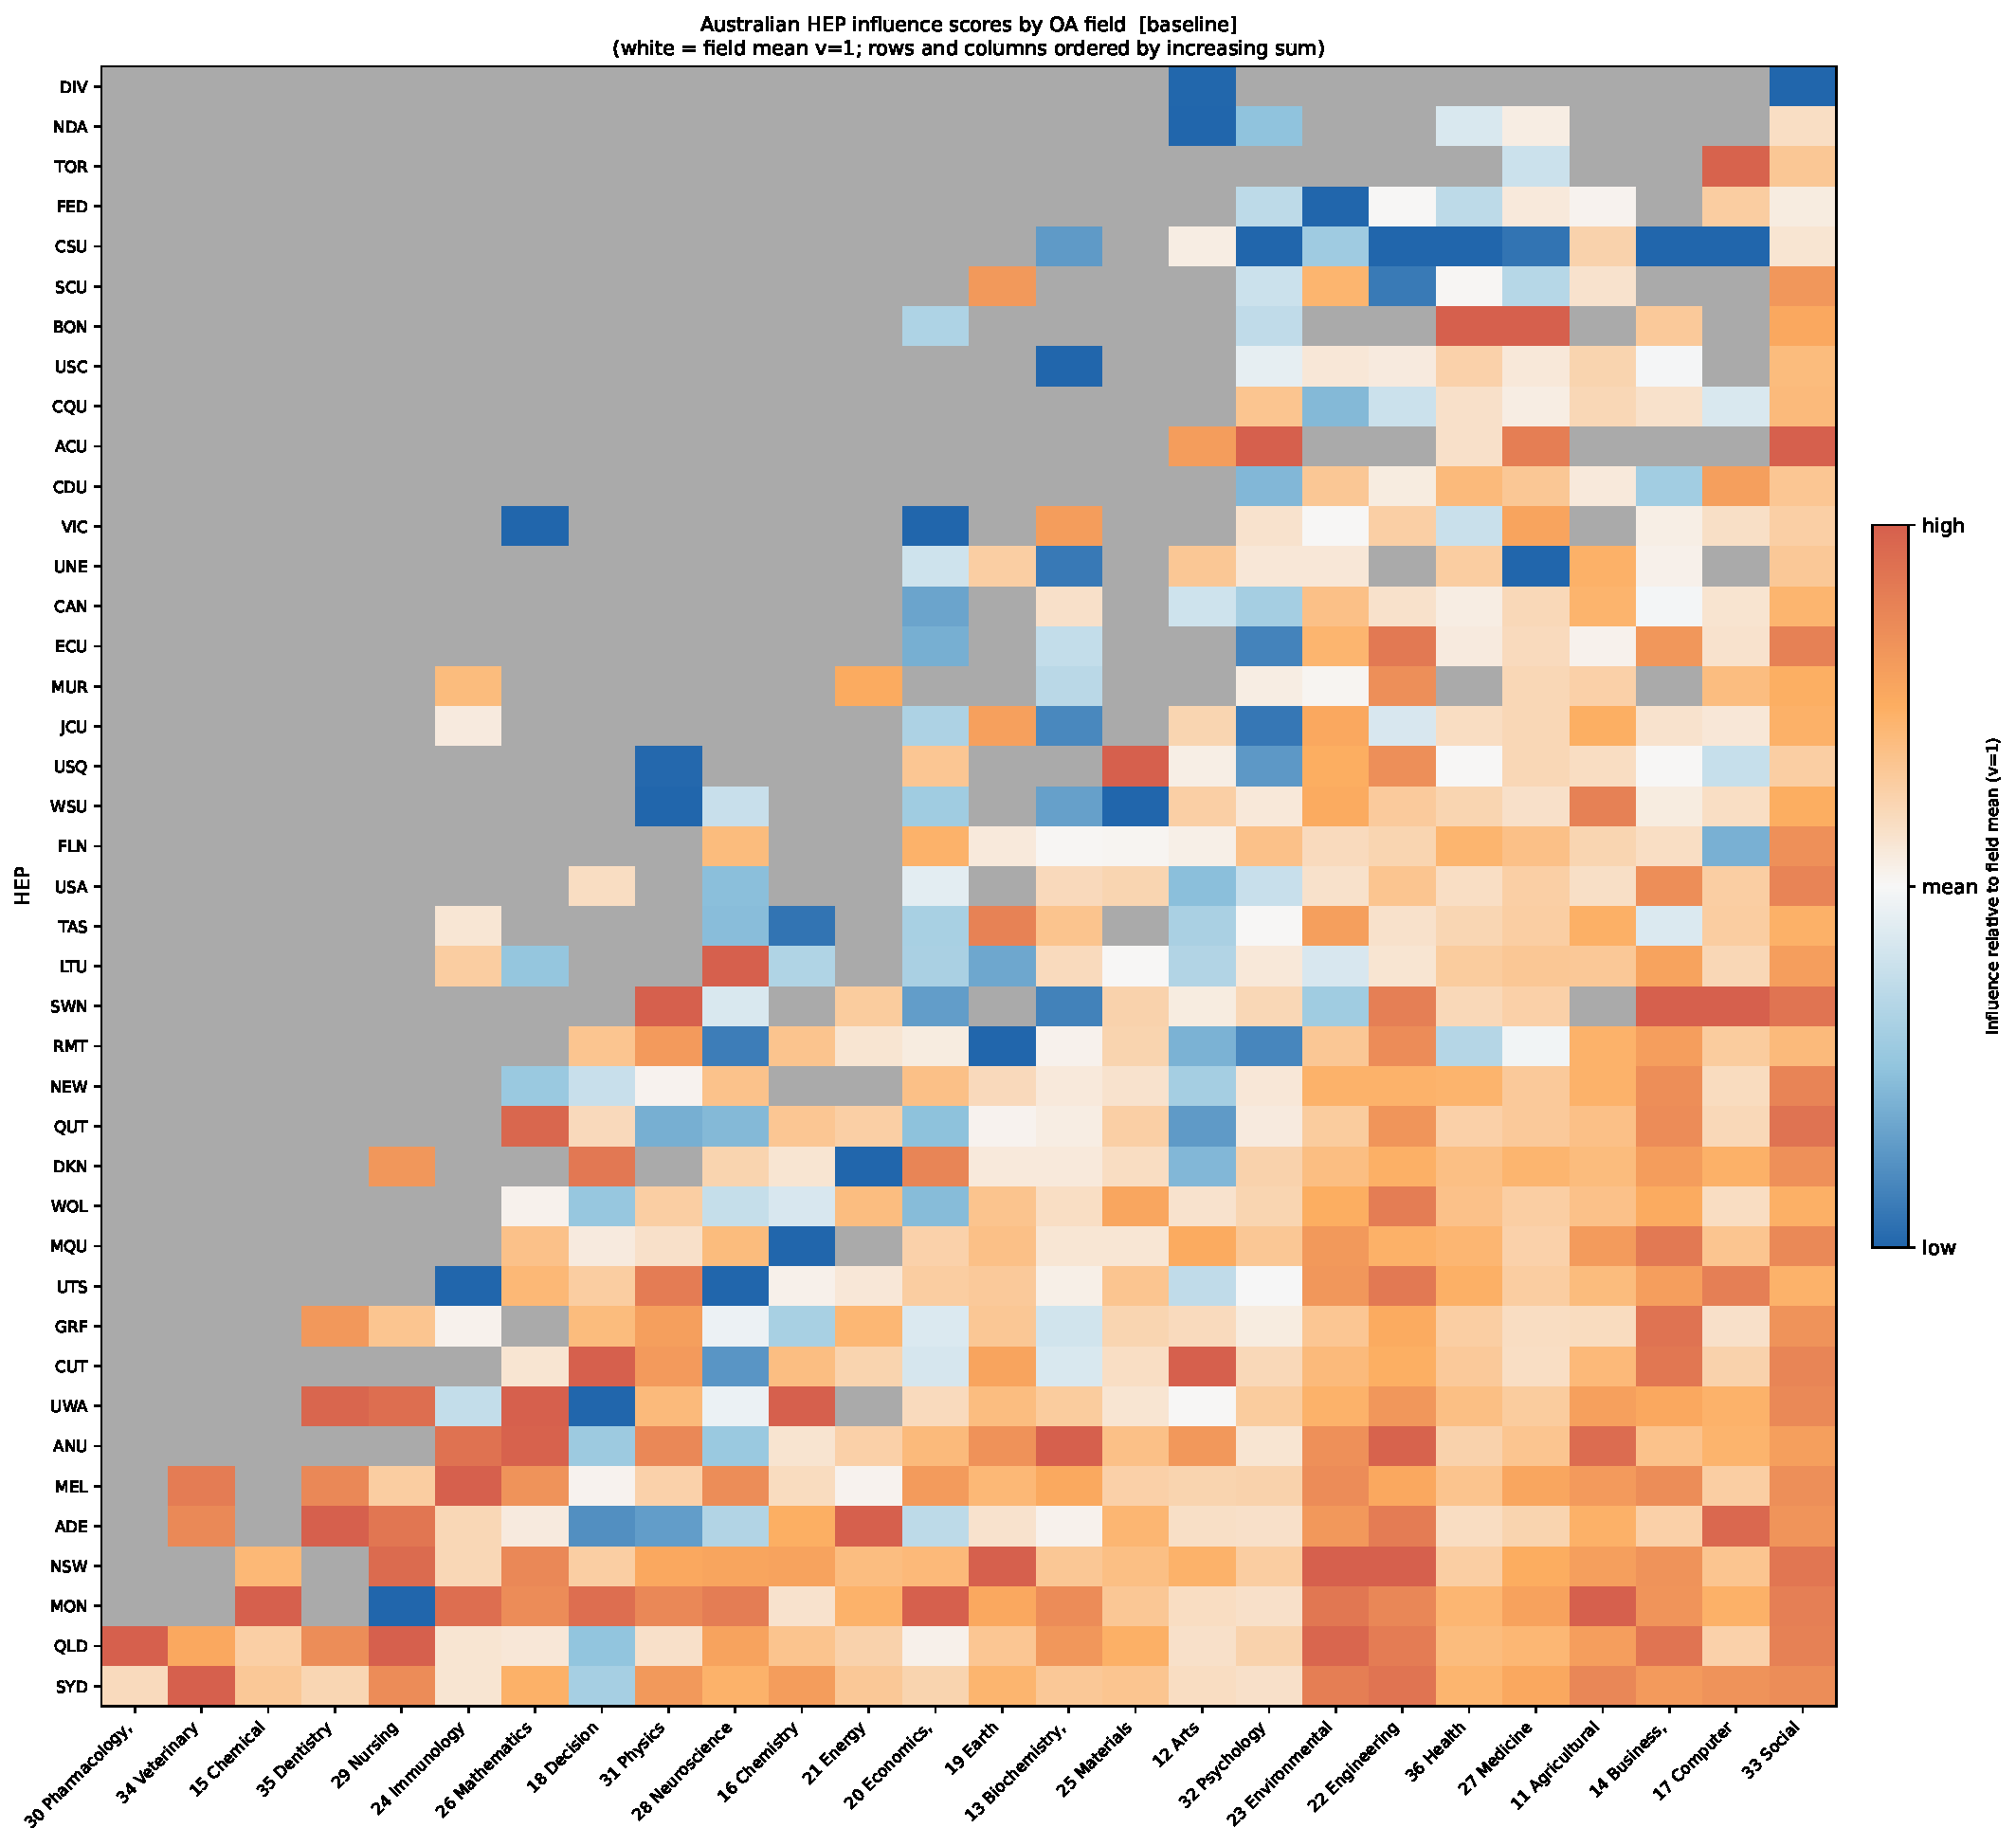
\includegraphics[width=\textwidth]{figures/fig2_hep_heatmap_fields.pdf}
\caption{Heatmap of Australian Higher Education Provider research influence scores ($v_I$) across 26 disciplines (2020--2024 census window). Cell colors range from blue ($v_I < 1.0$, below global mean) through white ($v_I = 1.0$, world average) to orange/red ($v_I > 1.0$, high research intensity). Institutions and disciplines are clustered by total influence.}
\label{fig:hep_heatmap}
\end{figure}

\begin{table}[htbp]
\centering
\small
\caption{Institutional Influence Scores ($v_I$) for Leading Australian Universities across the Five Broad Disciplines (World Average = 1.0).}
\label{tab:hep_summary}
\begin{tabularx}{\textwidth}{l >{\raggedright\arraybackslash}X c cccccc}
\toprule
\textbf{Code} & \textbf{Institution} & \textbf{Group} & \textbf{MCS} & \textbf{PSE} & \textbf{LES} & \textbf{BHS} & \textbf{SSH} & \textbf{Mean $v_I$} \\
\midrule
MON & Monash University & Go8 & 2.00 & 1.86 & 2.03 & 1.79 & 2.35 & \textbf{2.01} \\
SYD & University of Sydney & Go8 & 2.35 & 1.96 & 1.70 & 1.70 & 2.21 & \textbf{1.98} \\
SWN & Swinburne University of Technology & Non & 3.20 & 1.89 & 1.11 & 1.40 & 2.12 & \textbf{1.94} \\
ADE & University of Adelaide & Go8 & 2.92 & 1.95 & 1.38 & 1.38 & 1.96 & \textbf{1.92} \\
NSW & University of New South Wales & Go8 & 1.70 & 1.99 & 1.78 & 1.68 & 2.40 & \textbf{1.91} \\
UTS & University of Technology Sydney & ATN & 2.80 & 1.99 & 1.47 & 1.32 & 1.89 & \textbf{1.89} \\
ACU & Australian Catholic University & Non & 1.12 & -- & 1.55 & 1.86 & 2.92 & \textbf{1.86} \\
QLD & University of Queensland & Go8 & 1.68 & 1.96 & 1.76 & 1.58 & 2.24 & \textbf{1.85} \\
ANU & Australian National University & Go8 & 2.03 & 1.79 & 1.93 & 1.43 & 1.97 & \textbf{1.83} \\
MEL & University of Melbourne & Go8 & 1.66 & 1.61 & 1.76 & 1.73 & 2.16 & \textbf{1.79} \\
DKN & Deakin University & ATN & 2.08 & 1.45 & 1.33 & 1.56 & 2.19 & \textbf{1.72} \\
UWA & University of Western Australia & Go8 & 1.84 & 1.83 & 1.38 & 1.39 & 2.11 & \textbf{1.71} \\
TOR & Torrens University Australia & Non & 3.15 & -- & -- & 0.78 & 1.11 & \textbf{1.68} \\
MQU & Macquarie University & Non & 1.74 & 1.47 & 1.43 & 1.40 & 2.22 & \textbf{1.65} \\
QUT & Queensland University of Technology & Non & 1.53 & 1.69 & 1.39 & 1.39 & 2.09 & \textbf{1.62} \\
BON & Bond University & Non & -- & 1.15 & 0.49 & 2.30 & 2.43 & \textbf{1.59} \\
WOL & University of Wollongong & Non & 1.38 & 1.75 & 1.43 & 1.34 & 2.02 & \textbf{1.59} \\
CUT & Curtin University & ATN & 1.46 & 1.62 & 1.41 & 1.22 & 2.14 & \textbf{1.57} \\
NEW & University of Newcastle & Non & 1.32 & 1.54 & 1.42 & 1.40 & 2.16 & \textbf{1.57} \\
USA & University of South Australia & ATN & 1.59 & 1.60 & 1.36 & 1.37 & 1.88 & \textbf{1.56} \\
MUR & Murdoch University & IRU & 1.85 & 1.82 & 0.96 & 1.21 & 1.65 & \textbf{1.50} \\
ECU & Edith Cowan University & Non & 1.29 & 1.96 & 1.33 & 1.14 & 1.77 & \textbf{1.50} \\
RMT & RMIT University & ATN & 1.64 & 1.73 & 1.35 & 1.03 & 1.65 & \textbf{1.48} \\
CDU & Charles Darwin University & IRU & 2.32 & 1.01 & 1.21 & 1.49 & 1.37 & \textbf{1.48} \\
GRF & Griffith University & IRU & 1.35 & 1.62 & 1.25 & 1.21 & 1.92 & \textbf{1.47} \\
\bottomrule
\end{tabularx}
\end{table}


Several pivotal empirical findings emerge from this national analysis:

\begin{enumerate}
    \item \textbf{Comprehensive Excellence among the Group of Eight (Go8)}:
    All eight Go8 members achieve overall mean influence scores between $1.71$ and $2.01$, indicating that their research output attracts 70\% to 100\% more global prestige per unit than the world baseline. Monash University (MON, mean $v_I = 2.01$), the University of Sydney (SYD, $v_I = 1.98$), UNSW Sydney (NSW, $v_I = 1.91$), and the University of Adelaide (ADE, $v_I = 1.92$) exhibit broad-based intensity exceeding $1.6$ across all five macro-disciplines.
    
    \item \textbf{Specialized High-Intensity Clusters in the ATN and Non-Go8 Universities}:
    Crucially, the size-independent intensity metric $v_I$ reveals world-leading excellence outside the traditional Go8 establishment. Swinburne University of Technology (SWN) and the University of Technology Sydney (UTS) record extraordinary intensity in \textit{Mathematics, Computing and Information Sciences} (MCS $v_I = 3.21$ and $2.80$, respectively), outperforming all comprehensive universities in computing. Both institutions also demonstrate premier status in \textit{Physical Sciences and Engineering} (PSE $v_I = 1.89$ and $1.99$).
    
    \item \textbf{High-Intensity Niche Performers}:
    Australian Catholic University (ACU) provides a compelling demonstration of the metric's utility. Despite possessing a modest total volume of publications, ACU achieves the nation's highest institutional score in \textit{Social Sciences, Humanities and Business} (SSH $v_I = 2.92$) and strong biomedical/nursing performance (BHS $v_I = 1.86$), driving a mean institutional intensity of $1.86$. Under traditional volume-dependent metrics, ACU's distinctive research quality is frequently obscured.
    
    \item \textbf{Mission-Specific Strengths in Regional Universities}:
    Universities in the Regional Universities Network (RUN) and Innovative Research Universities (IRU) display targeted disciplinary excellence. For example, Deakin University (DKN, mean $v_I = 1.72$) achieves world-class status in computing (MCS $v_I = 2.08$) and social sciences (SSH $v_I = 2.20$), while Charles Darwin University (CDU) demonstrates localized environmental research strength.
\end{enumerate}

\subsection{Cross-Country Comparative Context}

To demonstrate that the bipartite spectral framework functions robustly across distinct national governance structures, Figure~\ref{fig:country_heatmap} illustrates national institutional profiles for Australia alongside the United Kingdom and the United States.

\begin{figure}[htbp]
\centering
\begin{minipage}{0.48\textwidth}
    \centering
    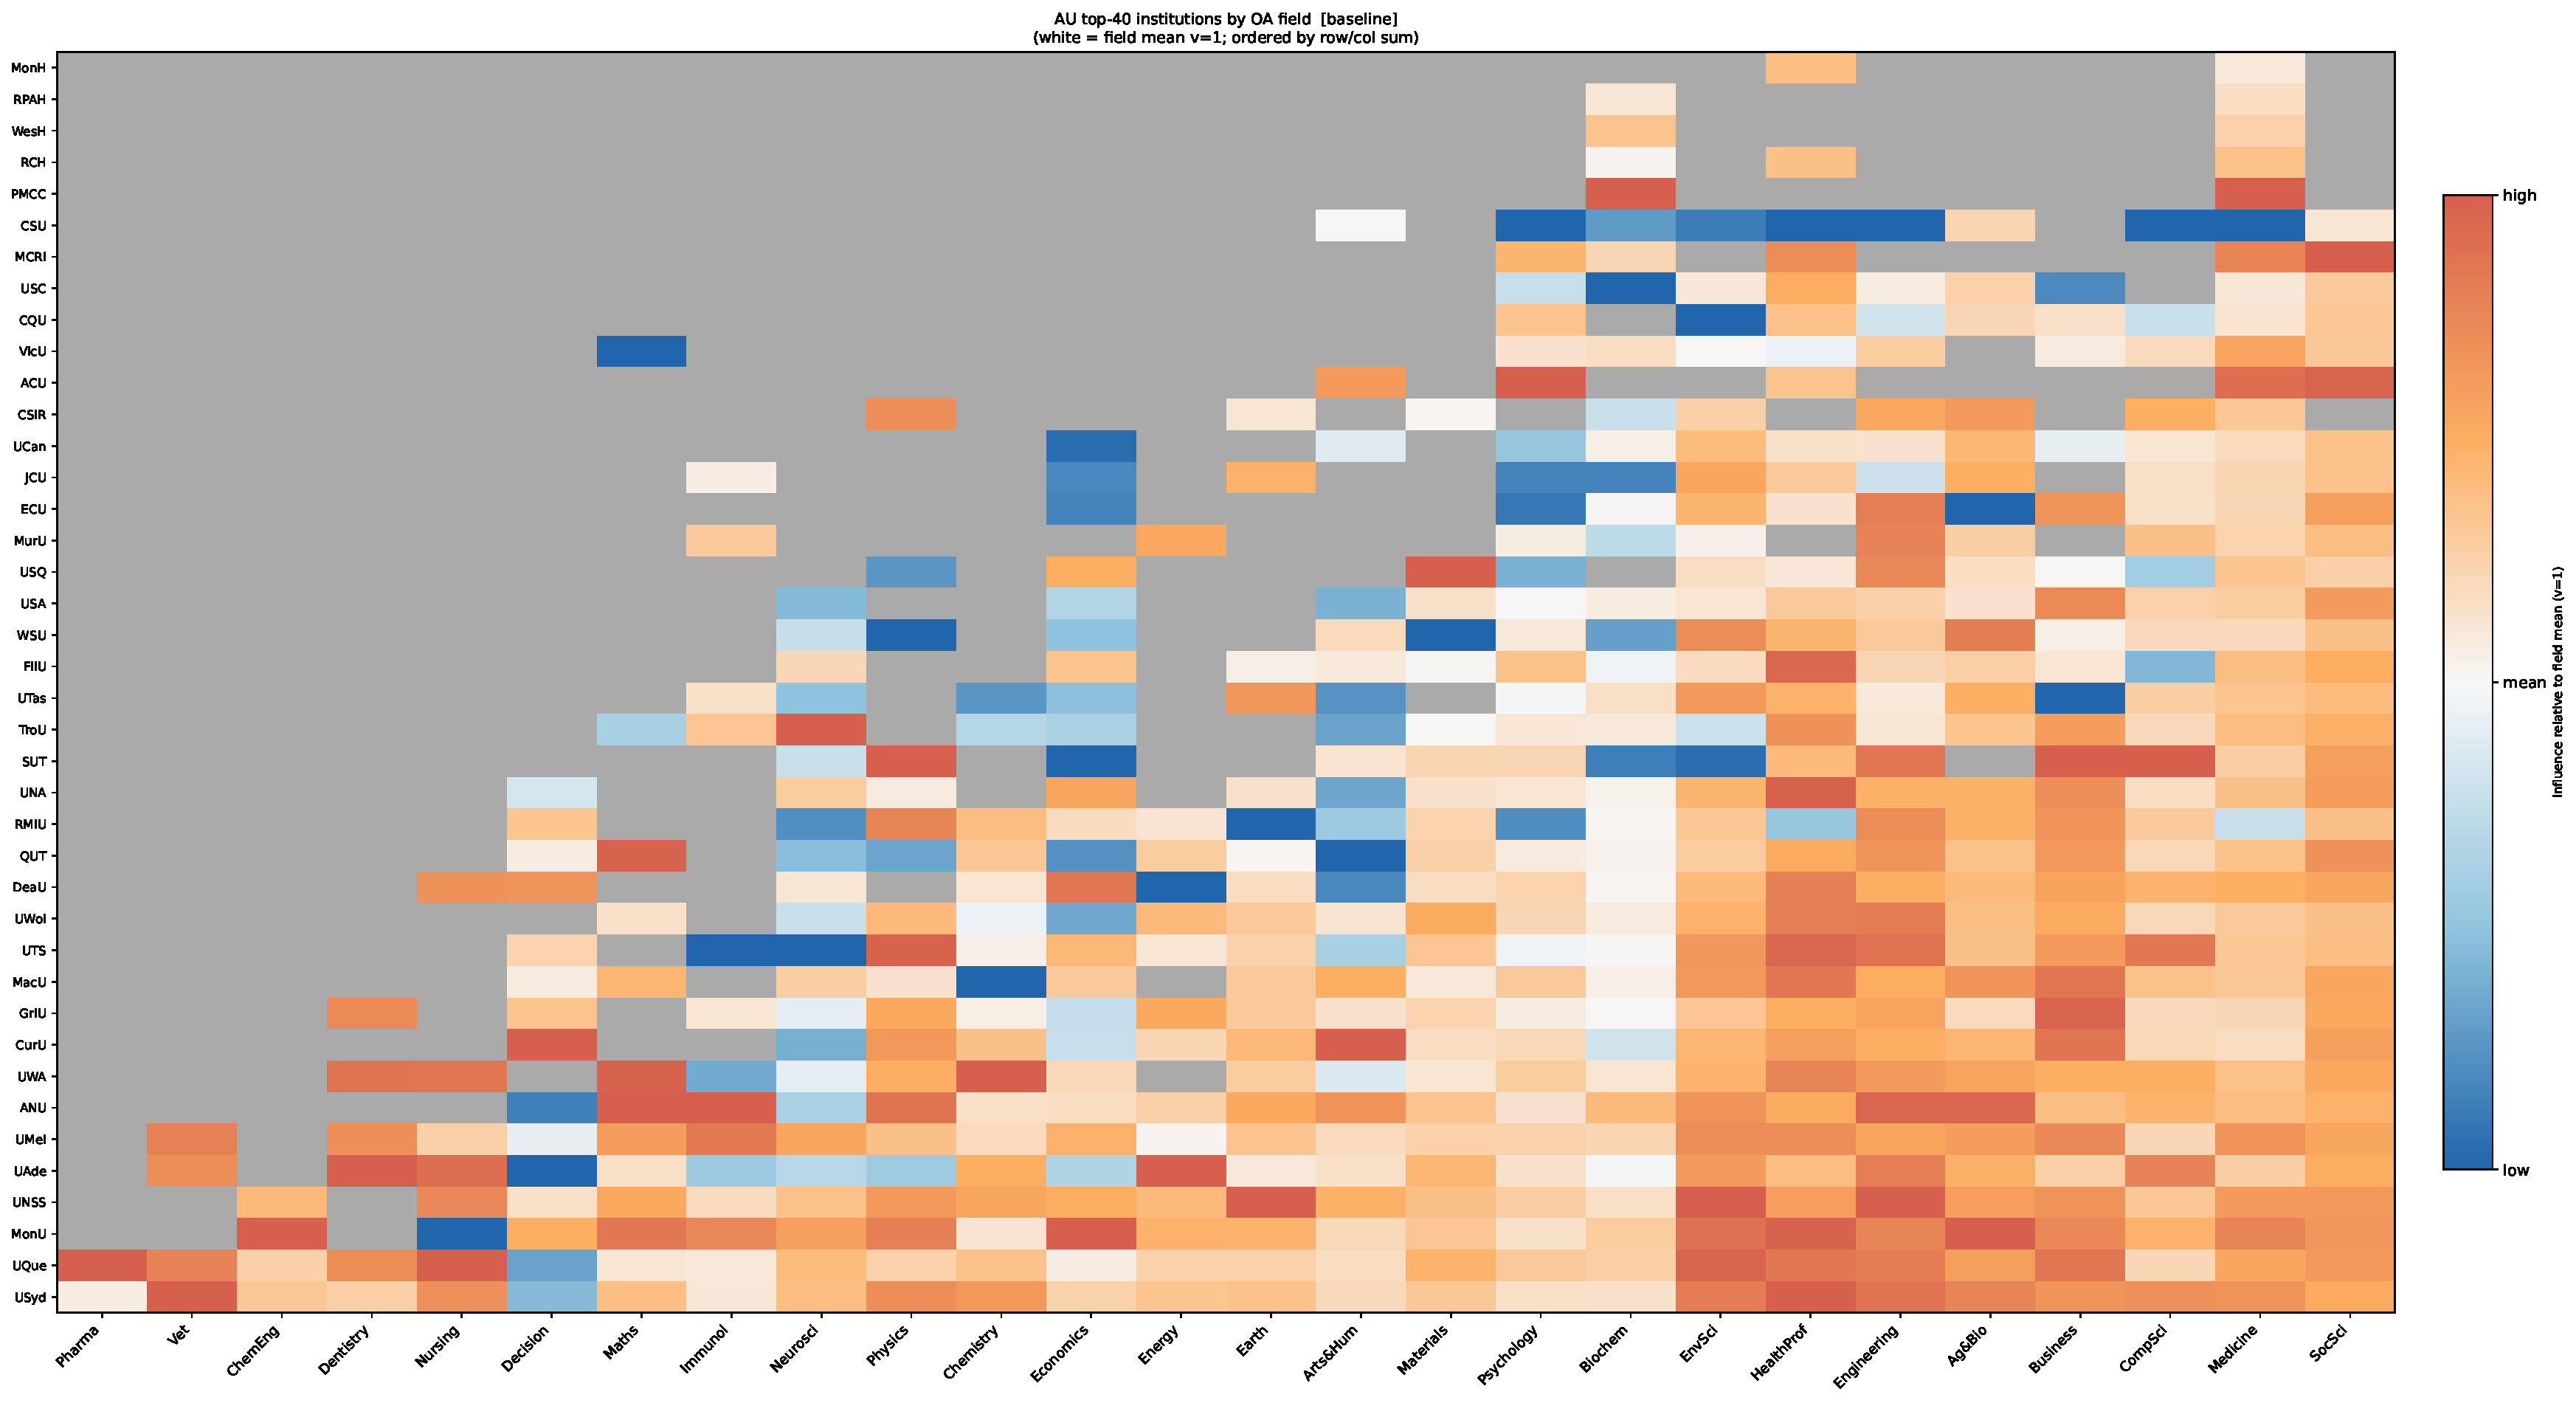
\includegraphics[width=\textwidth]{figures/fig3_country_heatmap_au.pdf}
    \caption*{(a) Australia (AU)}
\end{minipage}\hfill
\begin{minipage}{0.48\textwidth}
    \centering
    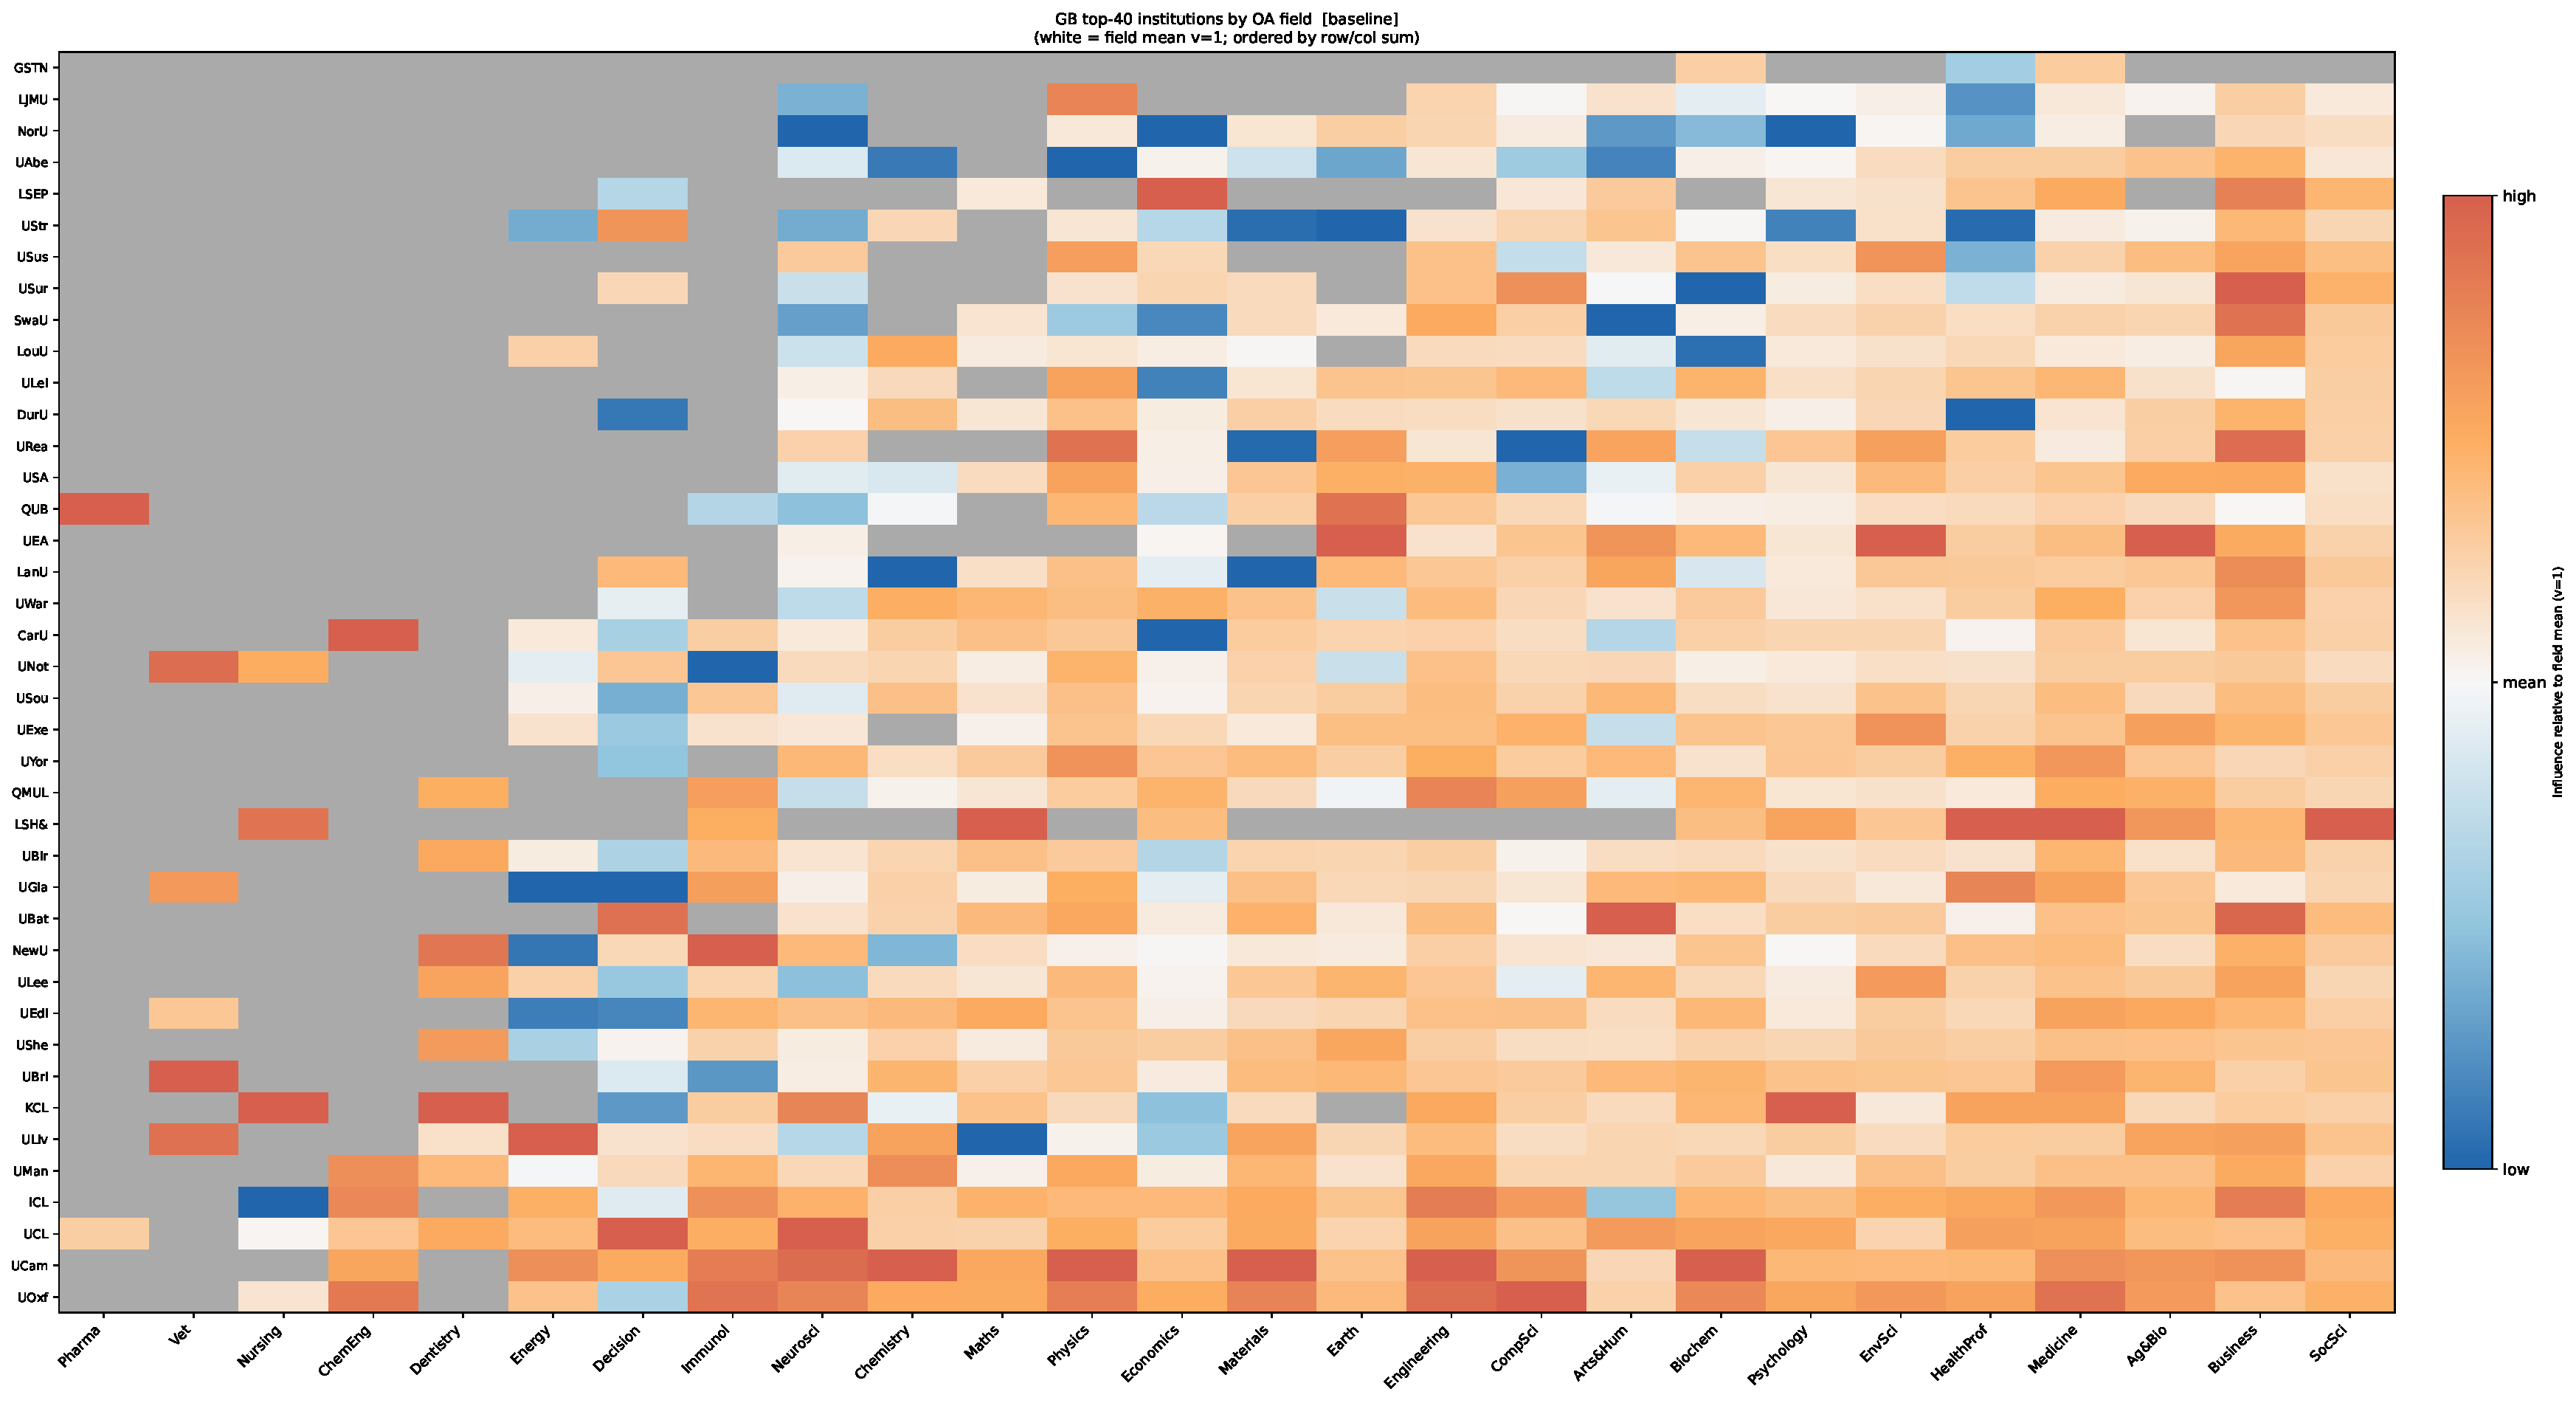
\includegraphics[width=\textwidth]{figures/fig3_country_heatmap_gb.pdf}
    \caption*{(b) United Kingdom (GB)}
\end{minipage}
\caption{Cross-country comparison of institutional research influence ($v_I$) across disciplines for top-ranked national universities in Australia and the United Kingdom.}
\label{fig:country_heatmap}
\end{figure}

The comparative profiles highlight a critical structural feature: unlike unipartite citation counts, which are inevitably dominated by large flagship multi-faculty campuses, bipartite prestige intensity illuminates specialized research institutes (e.g., medical research institutes and specialized polytechnics) with equal clarity across different national ecosystems.

\subsection{Algorithmic and Geopolitical Robustness}

A vital requirement for any national evaluation metric is stability against arbitrary boundary conditions and parameter specifications. We assess the resilience of the bipartite spectral ranking across two major dimensions: parameter perturbation and geopolitical citation bloc restriction.

Table~\ref{tab:sensitivity_correlations} reports the Spearman rank correlation ($\rho_s$) between baseline institutional rankings and five systematic variants across the five broad disciplines.

\begin{table}[htbp]
\centering
\small
\caption{Algorithmic and Geopolitical Stability: Spearman Rank Correlation ($\rho_s$) of Institutional Influence ($v_I$) between Baseline and Variants across the Five Broad Disciplines.}
\label{tab:sensitivity_correlations}
\begin{tabularx}{\textwidth}{>{\raggedright\arraybackslash}X ccccc}
\toprule
\textbf{Model / Bloc Variant} & \textbf{MCS} & \textbf{PSE} & \textbf{LES} & \textbf{BHS} & \textbf{SSH} \\
\midrule
OECD+G20 Bloc & 0.985 & 0.985 & 0.990 & 0.989 & 0.992 \\
OECD+G20 excl. CN/IN/US & 0.941 & 0.903 & 0.960 & 0.953 & 0.976 \\
AU, CN, IN, US Only & 0.956 & 0.949 & 0.942 & 0.935 & 0.017 \\
Retention Threshold ($\tau=20$) & 0.993 & 0.998 & 0.998 & 0.999 & 0.994 \\
Full Citation Count ($\rho=1$) & 0.953 & 0.908 & 0.966 & 0.973 & 0.975 \\
Sentinel Model ($\epsilon=1$) & 0.817 & 0.732 & 0.760 & 0.562 & 0.833 \\
\bottomrule
\end{tabularx}
\end{table}


\begin{figure}[htbp]
\centering
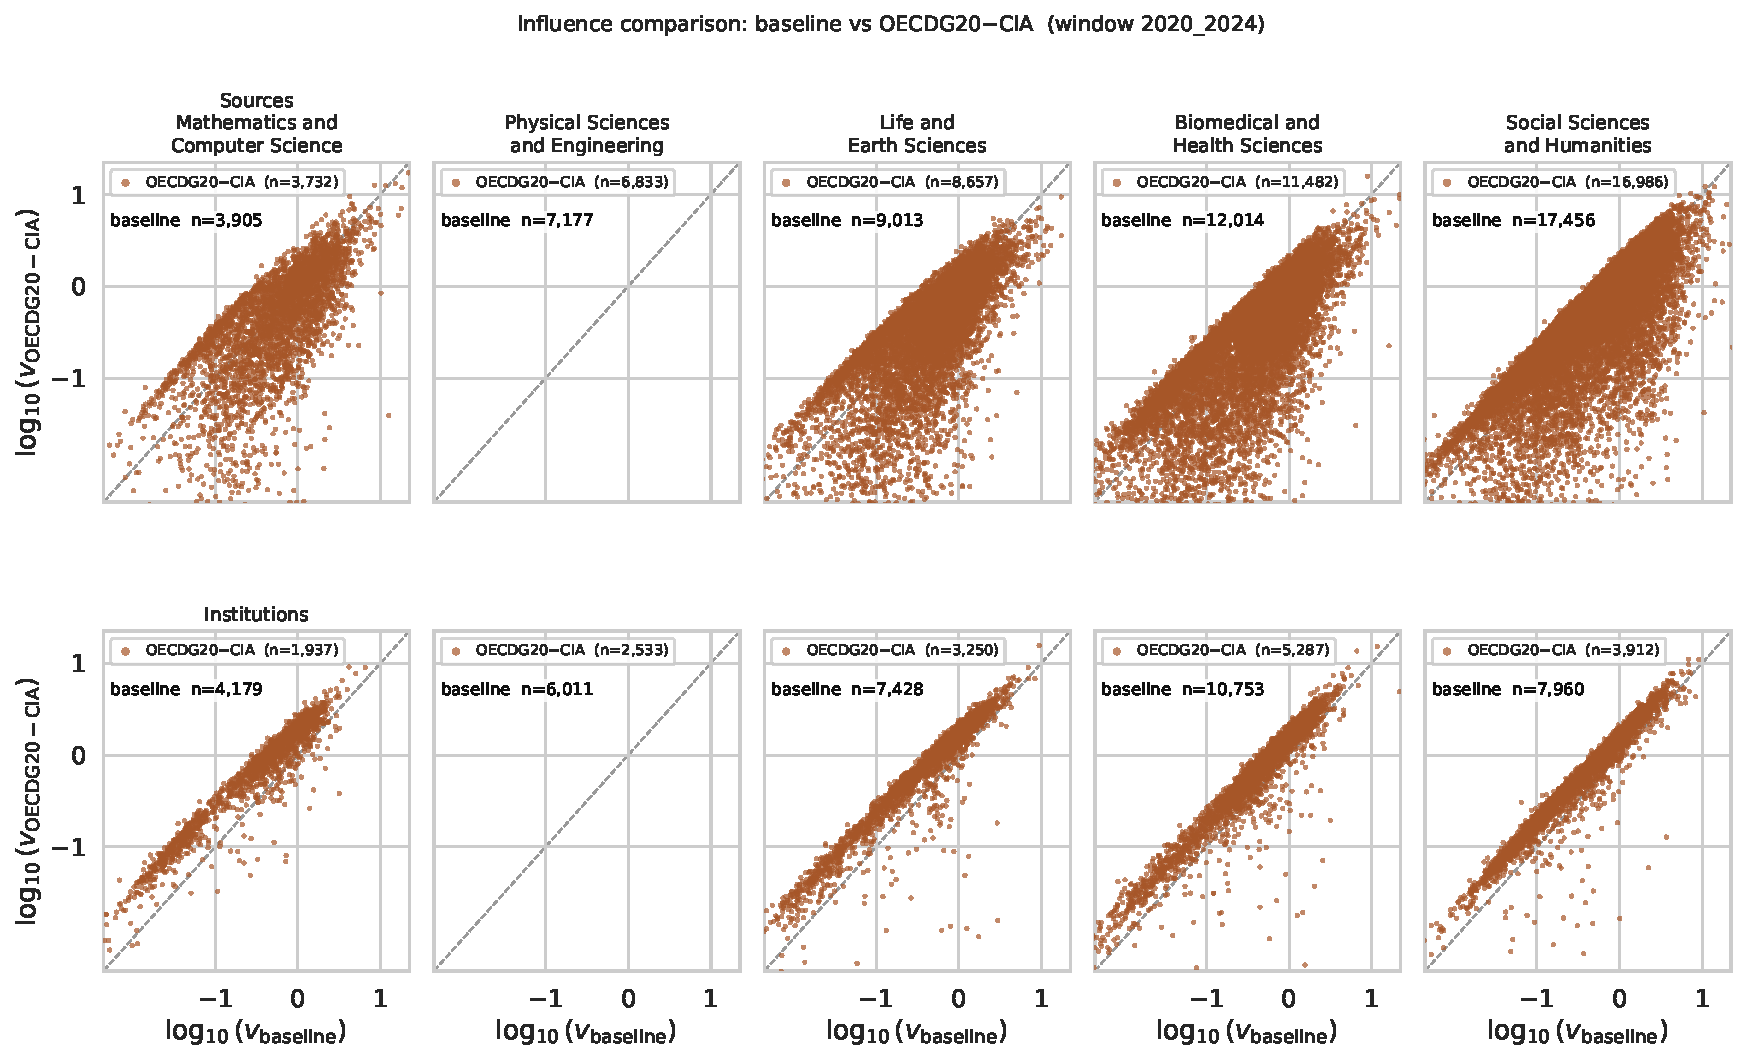
\includegraphics[width=0.88\textwidth]{figures/fig4_leiden_oecdg20cia_influence.pdf}
\caption{Stability of institutional influence ($v_I$) under geopolitical citation restriction: baseline global ranking ($x$-axis) versus the OECD+G20 excluding China, India, and the United States ($y$-axis) across sources (upper) and institutions (lower) for the five broad disciplines. The diagonal line denotes perfect invariance.}
\label{fig:bloc_stability}
\end{figure}

The empirical diagnostics demonstrate remarkable robustness:
\begin{itemize}
    \item \textbf{Retention Threshold Invariance ($\tau = 20$)}: Doubling the qualification threshold from 10 to 20 weighted works per year produces virtually identical institutional rankings, with Spearman rank correlations exceeding $0.993$ across all five disciplines.
    \item \textbf{Citation Multiplicity Weighting ($\rho = 1$)}: Replacing fixed-count citation weighting ($\rho = 0$) with full raw citation counts ($\rho = 1$) yields rank correlations between $0.908$ and $0.975$, proving that the bipartite projection is not hypersensitive to citation density normalization.
    \item \textbf{Geopolitical Bloc Stability}: When citations are restricted exclusively to the OECD+G20 bloc, institutional rank correlations exceed $0.985$ across all disciplines. Even when the world's three largest publishing powers (China, India, and the United States) are simultaneously excluded from the citation network (OECDG20-CIA), the rank correlation remains above $0.903$ in STEM and $0.976$ in SSH. As visualized in Figure~\ref{fig:bloc_stability}, institutions align tightly along the diagonal identity axis.
\end{itemize}

An instructive exception appears in the CIAA variant (AU, CN, IN, US only) within Social Sciences and Humanities ($\rho_s = 0.017$). In SSH, Chinese and Indian domestic citation networks operate in distinct linguistic and localized paradigms; restricting the entire world to this 4-country bloc severs the European, Commonwealth, and Latin American citation exchanges that anchor global social science discourse. This divergence affirms that the model sensitively captures genuine sociological realities rather than imposing a monolithic mathematical artifact.

% ---------------------------------------------------------------
\section{Discussion and Policy Implications}
\label{sec:discussion}
% ---------------------------------------------------------------

\subsection{A Modern Pathway for National Research Evaluation}

The findings presented in this study offer a direct, practical response to the core recommendations of the 2023 independent review of the Australian Research Council \citep[\textit{Trusting Australia's Ability};][]{sheil2023trusting} and the Australian Universities Accord \citep{accord2024final}: namely, that Australia should transition away from burdensome, submission-heavy retrospective evaluation exercises toward an agile, data-driven framework grounded in transparent global metrics.

By utilizing the open scholarly graph provided by OpenAlex \citep{priem2022openalex}, the bipartite spectral model eliminates the extensive administrative overhead that characterized ERA rounds---where university research offices spent months cleaning institutional rosters, verifying four-digit FOR codes, and assembling bespoke publication portfolios. Because the bipartite framework continuously computes institutional influence $v_I$ directly from published scholarly artifacts, national funding councils and higher education ministries can monitor disciplinary research intensity dynamically, transparently, and reproducibly, adhering closely to the principles of the Leiden Manifesto \citep{hicks2015leiden} and the Metric Tide \citep{wilsdon2015metric}.

\subsection{Structural Advantages for University Ecosystems}

Deploying a size-independent prestige intensity metric ($v$) yields profound structural benefits for national research strategy:

\begin{enumerate}
    \item \textbf{Equitable Recognition Across University Mission Groups}:
    Traditional university rankings and volume-weighted funding formulae create a powerful structural bias toward large, legacy multi-faculty universities with vast capital endowments \citep{docampo2015effect, docampo2017academic}. In contrast, the intensity metric $v_I$ reveals that technological universities (e.g., Swinburne and UTS in computer science) and specialized universities (e.g., ACU in social sciences and nursing) frequently achieve world-leading research intensity. National policy bodies can thus support diversity of mission and reward targeted excellence rather than incentivizing institutional homogenization.
    
    \item \textbf{Mitigating Metric Gaming and Journal Cartels}:
    Because the spectral algorithm solves for the mutual reinforcement of publishing channels and authoring institutions, it is inherently resistant to the known pathologies of unipartite metrics. An editor attempting to inflate a journal's impact factor via coercive self-citation does not alter the institutional prestige vector $\pi_I$; conversely, paper-mill publications in low-tier open-access venues carry minimal weight in the Breiger projection because those sources fail to attract citations from premier institutions.
    
    \item \textbf{Policy Alignment via the AREA5 Taxonomy}:
    By establishing an audited bridge to the ANZSRC FOR 2020 standard, the framework speaks directly to national policy portfolios. Maintaining computing and information sciences (MCS) as an independent macro-discipline provides clear visibility into national AI and digital capabilities, while aligning veterinary science with agriculture (LES) reflects authentic institutional structures in Australian universities.
\end{enumerate}

\subsection{Limitations and Future Directions}

While the bipartite spectral methodology resolves primary dilemmas in bibliometric evaluation, several methodological considerations remain:

\begin{itemize}
    \item \textbf{Humanities and Creative Arts (HASS)}: While OpenAlex has substantially expanded coverage of books, book chapters, and monographs (reflected in our 8-type corpus), scholarly communication in the creative arts, literature, and regional history continues to rely on non-traditional research outputs (NTROs) and regional publisher ecosystems that accrue citations slowly. For these disciplines, bipartite spectral status should serve as a contextual complement to peer review rather than an exclusive evaluative determinant.
    \item \textbf{Indigenous Research Recognition}: As documented in our taxonomy analysis, global automated topic hierarchies do not currently isolate Indigenous scholarship into a standalone branch. Given the vital national importance of ANZSRC Division 45 (\textit{Indigenous Studies}), assessing Indigenous research leadership requires dedicated, community-grounded frameworks that evaluate cultural authority, community benefit, and indigenous data sovereignty alongside standard bibliometric metrics.
    \item \textbf{Subfield and Meso-Level Disaggregation}: The current framework operates successfully at both the 5-area macro level and the 26-field level. A logical next step is extending the spectral machinery downward into OpenAlex's ~294 subfields to expose hyper-specialized subdisciplinary strengths (e.g., distinguishing quantum computing from software engineering).
\end{itemize}

\subsection{Conclusion}

The bipartite source/institution spectral ranking model establishes an equitable, mathematically rigorous, and policy-aligned paradigm for national research evaluation. By formalizing scientific status as a mutual reinforcement between scholarly venues and research institutions, and normalizing prestige by publication volume, the framework delivers an evidence-based assessment of research quality that decouples institutional size from intellectual influence. In a post-ERA environment, this methodology provides higher education authorities with an open, reproducible, and robust instrument for benchmarking national research capability on the world stage.


\bibliographystyle{../spbasic}
\bibliography{references,../MyLibrary}
\end{document}
